\chapter{Grundlagen}

\section{Testumgebungen im autonomen Fahren}
Um die Sicherheit und Zuverlässlichkeit von autonomen Fahrsystemen zu gewährleisten, müssen diese umfassend getestet werden. 
Dabei werden verschiedene Testumgebungen eingesetzt um die verschiedenen Anforderungen an die Systeme zu prüfen. 

\begin{itemize}
    \item Software-in-the-Loop (SIL) \newline
            Die zu prüfende Software wird in einer Simulationsumgebung getestet, wobei die Hardware-Komponenten des Fahrzeug simuliert werden. 
            Ziel ist es Fehler in der Software durch verschiedene Testszenarien frühzeitig zu identifizieren und zu beheben.
            Auf dieser Ebene ist das wiederholte Testen aufgrund von benötigter Zeit und Rechenleistung am günstigsten, da zum Beispiel schneller als in Echtzeit getestet werden kann. 
            Deshalb wird versucht möglichst viele Tests auf dieser Ebene durchzuführen.
    \item Hardware-in-the-Loop (HIL) \newline
            Bei HIL-Tests wird reale Zielhardware der Fahrzeuge wie Steuergeräte und Sensoren in die Simulation eingebunden. 
            So kann die Interaktion zwischen Software und Hardware unter kontrollierten Bedingungen relativ realitätsnah getestet werden.
    \item Vehicle-in-the-Loop (VIL) \newline
            VIL-Tests testen reale Fahrzeuge durch Fahrzeugtests im Verkehr, auf Teststrecken oder im Teststand. 
            Hier wird das komplette Zusammenspiel aller Software und Hardware-Komponenten im Fahrzeug geprüft.
            Diese Tests sind am aufwändigsten und teuersten, da sie reale Fahrzeuge sowie Testumgebungen benötigen.
\end{itemize}
\section{Klassifikation von Testszenarien im autonomen Fahren}
Testszenarien im Kontext des autonomen Fahrens können in zwei Kategorien unterteilt werden:
\begin{itemize}
    \item \textbf{Abstrakte Szenarien:}
    Beschreiben die Verkehrssituation auf einem hohen Grad an Abstraktion. Sie definieren die grundlegenden Anforderungen und die Randbedingungen ohne spezifische numerische Werte.
    \newline Beispiel Überholszenario: Ein Fahrzeug V1 überholt das VUT.
    \item \textbf{Konkrete Szenarien:}
    Stellen eine vollständige Instanziierung eines abstrakten Szenarios dar. Sie beschreiben die Anforderungen in präzise, quantifizierbaren Daten. Dazu gehören unter anderem die Positionen, Geschwindigkeiten und Zeitpunkte.
    \newline Beispiel Überholszenario: Auf einer dreispurigen Autobahn startet das Fahrzeug V1 mit $v = 25 \frac{\text{m}}{\text{s}}$ auf der linken Spur. Das VUT startet $15 \text{m}$ davor auf der mittleren Spur mit $v = 20 \frac{\text{m}}{\text{s}}$. Nach $5$ Sekunden wechselt das Fahrzeug V1 auf die mittlere Spur vor das VUT.
\end{itemize}
Diese Unterscheidung ist entscheidend für die automatisierte Szenariengenerierung, da aus allgemeinen Vorgaben eine Vielzahl spezifischer Tests abgeleitet werden können.

\section{OpenSCENARIO als Standard zur Beschreibung von Testszenarien}



Ein Standard für die Beschreibung von Testszenarien für autonomes Fahren ist OpenSCENARIO, welches durch die ASAM (Association for Standardization of Automation and Measuring Systems) entwickelt wurde.
Im Laufe der Zeit wurden verschiedene Versionen veröffentlicht, frühe Versionen basieren auf XML, was die Erstellung und Wartung von Szenarien aufgrund des Umfangs und dem Detailgrad komplex macht.
Später wurde OpenSCENARIO DSL entwickelt, eine domänenspezifische Sprache, die eine einfachere und intuitivere Beschreibung von Szenarien ermöglicht.

\begin{figure}[h]
    \centering
    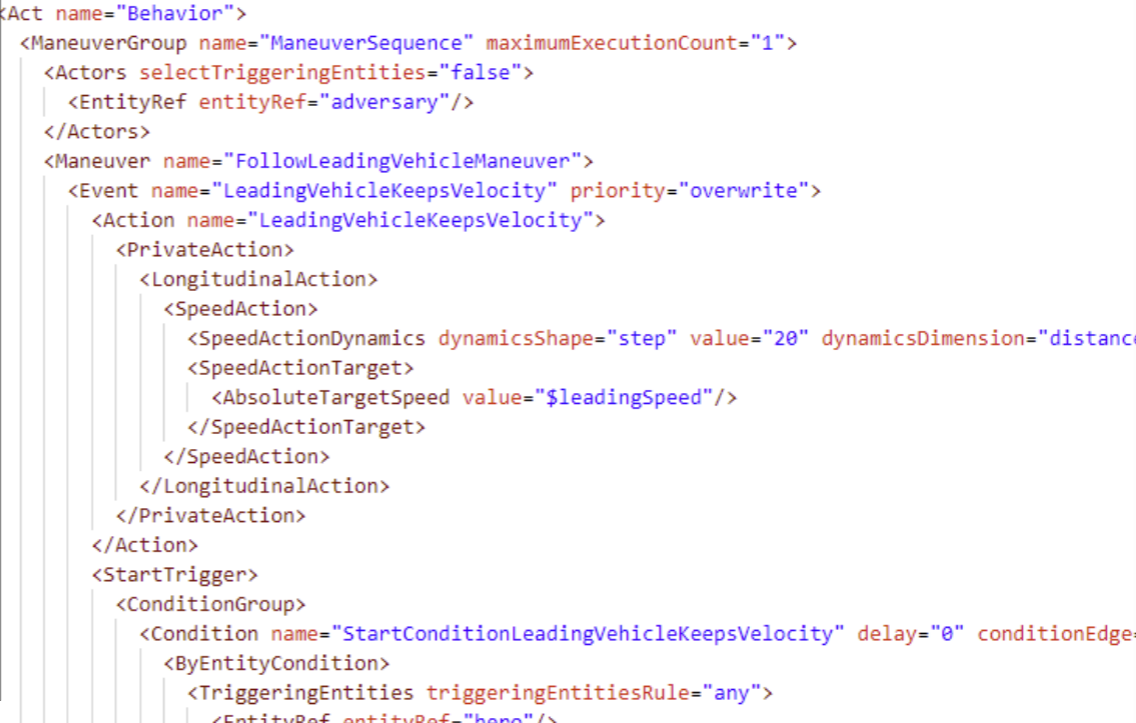
\includegraphics[width=0.85\linewidth]{contents/figures/openscenario_xml.png}
    \caption{OpenSCENARIO XML Beispiel \cite{EinfuehrungIntegrationsprojekt}}
    \label{fig:osl-xml}
\end{figure}

Abbildung \ref{fig:osl-xml} zeigt einen beispielhaften Ausschnitt eines OpenSCENARIO XML Szenarios.
Das Szenario ist dabei in \glqq Acts\grqq{} gegliedert, welche jeweils eine Menge von Aktionen definieren.
Diese werden durch Subtypen definiert und enthalten unter anderem Informationen über die beteiligten Akteure, deren Start- und Endzeitpunkt sowie die Art der Aktion.
Damit ist ein genaues Beschreiben von Testszenarien möglich, allerdings ist die XML-Syntax sehr umfangreich und für Menschen unübersichtlich, dafür aber einfach maschinenlesbar.



In Abbildung \ref{fig:osl-dsl} ist ein weiteres Szenario mit OpenSCENARIO DSL dargestellt.
Die DSL-Syntax ist deutlich kompakter und einfacher lesbar als die XML Syntax, was die Erstellung und Wartung von Szenarien erleichtert.
Es werden zwei Fahrzeuge definiert, welche sich auf einer Straße befinden und eine Überholsituation durchführen sollen.
Dabei sind im Sinne eines abstrakten Szenarios beispielsweise Intervalle definiert, in denen das Überholmanöver durchgeführt werden soll, sowie die Abstände, die zwischen den Fahrzeugen eingehalten werden sollen.
Allerdings wird das Szenario nur deklarativ beschrieben, enthält also keine Anweisungen zur Ausführung sondern dazu, welche Abläufe valide sind.
Ein automatisiertes Testen ist damit dadurch nicht ohne weiteres möglich, da ein Parsen der Syntax und eine Interpretation der Szenariobeschreibung notwendig ist. 

\begin{figure}[h]
    \centering
    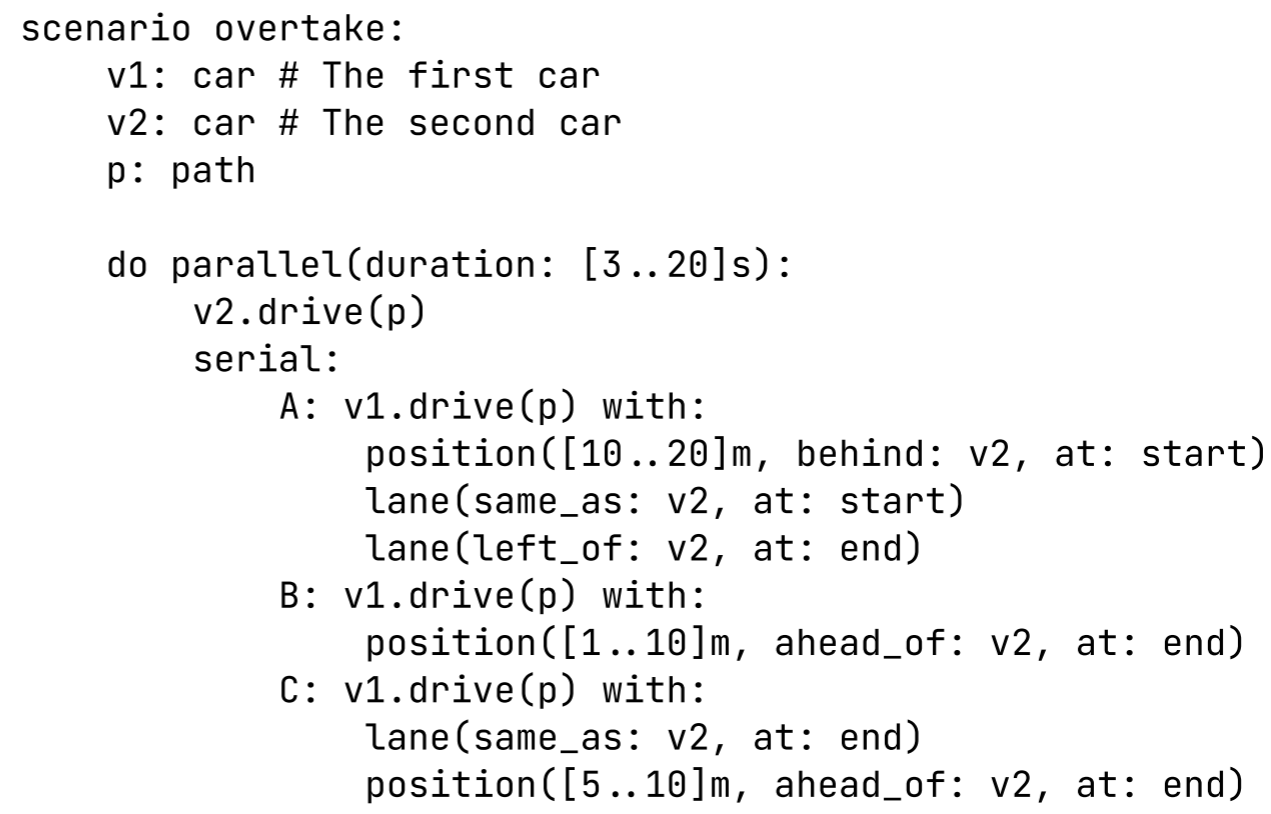
\includegraphics[width=0.6\linewidth]{contents/figures/openscenario_dsl.png}
    \caption{OpenSCENARIO DSL Beispiel \cite{EinfuehrungIntegrationsprojekt}}
    \label{fig:osl-dsl}
\end{figure}

\section{Eingesetzte Simulations-Engines im Rahmen dieser Arbeit}
Simulationsumgebungen sind ein zentrales Werkzeug im Bereich des autonomen Fahrens. Sie ermöglichen es, Verkehrssituationen unter kontrollierten Bedingungen nachzustellen und die entwickelten Verfahren zu testen. Abhängig vom jeweiligen Einsatzgebiet unterscheiden sich die Umgebungen vor allem im Grad der Abstraktion, in den bereitgestellten Funktionen und im benötigten Rechenaufwand. In den folgenden Abschnitten werden mit HighwayEnv sowie SUMO und dem dazugehörigen TraCI zwei Umgebungen vorgestellt, die in unserem Projekt verwendet werden.
\subsection{HighwayEnv}
HighwayEnv ist eine Open-Source-Simulationsumgebung für autonomes Fahren, welches auf der Basis von Gymnasium beziehungsweise OpenAI Gym entwickelt wurde \cite{highway-env}. Der Fokus liegt auf einer schnellen abstrahierten Simulation auf mehrspurigen Straßen und Autobahnen. Das Ziel dieser Simulationsumgebung ist die Entwicklung, Training und Evaluierung von Reinforcement-Learning-Algorithmen und Planungsverfahren im Bereich des autonomen Fahrens.

Technisch ist es mit Python implementiert und folgt einem modularen Aufbau, welche sich an der klassischen Agent-Environment-Schnittstelle aus dem Bereich des Reinforcement-Learnings bedient \cite{highway-env}. Die einzelnen Szenarien werden durch Environment-Klassen definiert, etwa highway-v0 (ein klassisches Autobahn-Szenario) oder roundabout-v0 (ein Kreisverkehr) \cite{highway-env}. Damit eine effiziente Simulation stattfinden kann nutzt es mittels eines kinematischen Modells eine vereinfachte Fahrzeugdynamik.

Bei der Fahrzeugmodellierung beschränkt sich HighwayEnv auf wesentliche Parameter, wie Position, Geschwindigkeit und Fahrtrichtung. Die Umgebungsmodellierung bietet mehrspurige Straßen, Fahrspurwechsel sowie unterschiedliche Verkehrsdichten \cite{highway-env}. Ein Agent kann beschleunigen, bremsen, die Spur wechseln oder seine aktuelle Bewegung beibehalten. Die im Reinfocement-Learning benötigte Belohnungsfunktion kann je nach Zielstellung beliebig angepasst werden, z.B. auf Sicherheit oder Effizienz. 

Der Fokus von HighwayEnv liegt vor allem auf abstrakten Szenarien und nicht hochrealistischen Simulationen. Es ist somit kein Ersatz für High-Fidelity-Simulatoren, wie CARLA. Zudem bietet es keine realistische Physik. Dadurch werden beispielsweise Fahrdynamiken oder Wetterbedingungen vernachlässigt. Der Vorteil von HighwayEnv liegt in den geringen Rechenkosten und ist somit geeignet für Experimente und Prototyping.
\subsection{Sumo und Traci}
Die Simulation of Urban MObility, kurz SUMO, ist ein Open-Source, mikroskopischer, straßenverkehrsbasierter Simulator, welcher vom Deutschen Zentrum für Luft- und Raumfahrt (DLR) entwickelt wird \cite{SUMO2018}. Das Ziel ist es Verkehrsflüsse und - dynamiken in realistischen Straßennetzwerken zu simulieren. Es untsertützt Einzel- sowie Massensimulationen von Fahrzeugbewegungen in Städten, Autobahnen und Mischverkehr.

Die Implementierungssprache ist im Kern C++. Zudem stehen Python-APIs zur Verfügung mit denen Erweiterungen möglich sind. Mikroskopisch bedeutet in diesem Fall, dass jedes Fahrzeug einzeln simuliert wird \cite{sumo_at_a_glance}. Die Straßennetze können aus realen Karten, wie OpenStreetMap importiert werden, sodass eine hohe Flexibilität geboten ist \cite{sumo_open_street_map}. Des Weiteren werden verschiedene Fahrzeugtypen von LKWs und Bussen über den PKW bis hin zum Fahrrad oder Fußgänger bereitgestellt.

Für die Fahrdynamik werden Car-Following-Modelle wie das Krauß-Modell genutzt \cite{sumo_car_following}. Darüber hinaus finden Lane-Change-Modelle Anwendung. Innerhalb der Verkehrssteuerung können Amplen, Zuflussregelungen oder auch Stauszenarien simuliert werden. Des Weiteren gibt es eine eingebaute Routenplanung sodass Fahrzeuge entweder feste Routen folgen oder auf Basis von dynamischen Routing-Algorithmen gesteuert werden können \cite{sumo_vehicles}. Im Bereich der Auswertungen werden verschiedene detaillierte Statistiken im Bezug auf Reisezeiten, Emissionen oder Staus geliefert.

Die Einsatzbereiche von SUMO reichen von der Verkehrsforschung, wobei Verkehrsflüsse, Engpässe oder Infrastrukturmaßnahmen untersucht werden bis hin zur Stadtplanung und Mobilitätskonzepten bei denen Szenarien, wie Car-Sharing oder ÖPNV, simuliert werden \cite{SUMO2018}. Zudem kann es auch im Bereich des autonomen Fahrens als Testumgebung für Entscheidungs- und Koordinationsstrategien dienen.

Im Gegensatz zu HighwayEnv benötigt SUMO bei sehr großen Netzen eine hohe Rechenlast. Es bietet zudem auch keine High-Fidelity, da auch hier ein vereinfachtes Fahrzeugmodell verwendet wird.

Mit dem Traffic Control Interface (TraCI) bietet das DLR eine Client-Server-Schnittstelle zur Echtzeitsteuerung und Abfrage von SUMO-Simulationen \cite{sumo_traci}. Dies erlaubt die dynamische Interaktion mit einer laufenden SUMO-Simulation. Dabei kann ein lesender Zugriff zur Abfrage von Zuständen etwa der Position, Geschwindigkeit und Ampelphasen erfolgen. Darüber hinaus ist eine Manipulation der Simulation, indem beispielsweise Fahrzeuge hinzugefügt oder Routen verändert werden, möglich \cite{sumo_traci}. Dies erlaubt die Einbindung von externen Steuerungsalogrithmen z.B. Reinforcement-Learning oder Verkehrsmanagementsysteme.

\section{Behavioral Programming Paradigma}\label{sec:behavioral-programming}
Behavioral Programming (BP) ist ein sprachunabhängiges Programmierparadigma zur Entwicklung reaktiver Systeme\cite{Harel2012}.
Dabei steht die inkrementelle Spezifikation von Verhalten im Vordergrund, während klassische Kontrollflussentscheidungen in den Hintergrund treten\cite{Harel2012}.
BP wurde ursprünglich im Kontext der szenarienbasierten Programmierung entwickelt und später auch in Umgebungen wie Java (als \emph{BPJ}-Framework) und Python (als \emph{BPpy}) umgesetzt\cite{Harel2010}.
Die zentralen Bausteine dieses Paradigmas sind sogenannte \emph{Behavior Threads} (B-Threads), welche einzelne Verhaltensaspekte kapseln und nebenläufig ausgeführt werden\cite{Harel2010}.
Alle B-Threads kommunizieren ausschließlich über \emph{Ereignisse} und werden an definierten Synchronisationspunkten vom Laufzeitsystem koordiniert\cite{Harel2012}.

\subsection{Fokus auf Verhalten statt Kontrolle}\label{subsec:fokus-auf-verhalten-statt-kontrolle}
In BP wird jeder Systemaspekt als separates Verhalten (in einem eigenen B-Thread) implementiert, anstatt einen zentralen Ablaufplan zu programmieren.
Dadurch ergibt sich eine \emph{indirekte Steuerung}: Anstatt dass ein Modul direkt ein anderes aufruft oder steuert, beeinflussen sich die Verhaltensmodule nur über das Anbieten oder Verhindern von Ereignissen\cite{Harel2012}.
Dieses Prinzip erlaubt eine natürlichere Beschreibung von Anforderungen, das heißt es wird spezifiziert, was geschehen oder unterbleiben soll, ohne die Ausführung in Form von detailliertem Kontrollfluss explizit zu kodieren\cite{Harel2012}.
Die Auswahl des nächsten Systemschritts (Ereignisses) erfolgt zur Laufzeit durch das BP-Laufzeitsystem, das aus den von allen B-Threads vorgeschlagenen und gegebenenfalls gesperrten Ereignissen ein zulässiges Ereignis bestimmt und ausführt\cite{Harel2012}.
BP verlagert den Schwerpunkt der Programmierung somit von der Implementierung von Steuerungslogik hin zur Spezifikation von erwünschtem oder verbotenem Verhalten.

\subsection{B-Threads und ereignisgesteuerte Synchronisation}\label{subsec:b-threads-und-ereignisgesteuerte-synchronisation}
Ein B-Thread ist eine in sich geschlossene Verhaltenskomponente, typischerweise implementiert als unabhängiger Prozess (Thread, Coroutine o. Ä.), der wiederholt Ereignisse abgibt oder auf Ereignisse wartet.
Die Koordination aller B-Threads erfolgt an expliziten \emph{Synchronisationspunkten}.
Jeder B-Thread ruft eine Synchronisationsoperation (etwa \emph{sync}) auf, wobei er drei Kategorien von Ereignissen deklariert\cite{Harel2010}:
\begin{itemize}
  \item \textbf{Gewünschte Ereignisse} (\emph{requested events}): Ereignisse, die der Thread vorschlägt und bei deren Auftreten er fortgesetzt werden möchte.
  \item \textbf{Erwartete Ereignisse} (\emph{waited-for events}): Ereignisse, auf die der Thread passiv wartet.
  \item \textbf{Blockierte Ereignisse} (\emph{blocked events}): Ereignisse, die der Thread momentan verhindern möchte.
\end{itemize}

Sobald alle aktiven B-Threads ihren Synchronisationspunkt erreicht haben, sammelt das Laufzeitsystem alle vorgeschlagenen Ereignisse und wählt eines davon aus, das von mindestens einem B-Thread vorgeschlagen und von keinem B-Thread blockiert wurde\cite{Harel2012}.
Das ausgewählte Ereignis wird anschließend ausgelöst; alle B-Threads, die dieses Ereignis vorgeschlagen oder darauf gewartet haben, werden aufgeweckt und setzen ihre Ausführung bis zum nächsten Synchronisationspunkt fort\cite{Harel2012}.
B-Threads, die das Ereignis weder angefordert noch erwartet hatten, bleiben solange pausiert\cite{Harel2012}.
Falls mehrere vorgeschlagene Ereignisse gleichzeitig ausführbar sind, kann je nach Implementierung ein Prioritätenschema oder eine feste Rangfolge zur Anwendung kommen, um ein deterministisches Verhalten zu gewährleisten\cite{Harel2012}.
Anschließend erfolgt die nächste Synchronisation aller Threads, und der Zyklus wiederholt sich.
Dieses ereignisgesteuerte Synchronisationsverfahren stellt sicher, dass sich unabhängige Teilverhalten konsistent zu einem Gesamtablauf verweben, ohne dass eine zentrale Steuerlogik die einzelnen Schritte vorgibt.

\subsection{Modularität und Erweiterbarkeit}\label{subsec:modularitat-und-erweiterbarkeit}
Ein Hauptvorteil von BP ist die \emph{hohe Modularität} der Verhaltensbeschreibung und die einfache Erweiterbarkeit von Systemfunktionalität.
Neue Anforderungen können als zusätzliche B-Threads implementiert werden, was eine \emph{inkrementelle Entwicklung} ermöglicht, bei der bestehender Code kaum oder gar nicht geändert werden muss\cite{Harel2012}.
\newline
Das Hinzufügen oder Entfernen von Verhaltensmodulen entspricht dem Ein- oder Ausschalten von Szenarien, ohne unbeabsichtigte Seiteneffekte auf den übrigen Ablauf.
\newline
\newline
Alle Module interagieren ausschließlich über das gemeinsame Ereignis-Vokabular und kennen einander nicht direkt\cite{Harel2010}.
So kann beispielsweise in einem einfachen Wassermisch-System ein zusätzliches Verhalten (Interleave, abwechselndes Heiß- und Kalt-Zapfen) durch einen neuen B-Thread realisiert werden, der abwechselnd auf das eine Ereignis wartet und das andere blockiert, ohne die bestehenden B-Threads zu verändern\cite{Harel2012}.
\newline
\newline
BP unterstützt damit auch Konzepte wie die merkmalsorientierte Entwicklung (Feature-Oriented Development) und Produktlinien: Unterschiedliche Ausprägungen eines Systems können durch Konfiguration der Menge der aktiven B-Threads erzeugt werden\cite{Harel2012}.
Im Vergleich zu objektorientierten oder aspektorientierten Ansätzen vermeidet BP die strikte Trennung zwischen Basis- und Erweiterungslogik; stattdessen wirken alle Verhaltensmodule gleichberechtigt zusammen\cite{Harel2012}.
Darüber hinaus lässt sich BP mit anderen Programmierparadigmen kombinieren.
B-Threads teilen keinen gemeinsamen Zustand, sondern koordinieren sich ausschließlich indirekt über Ereignisse, was eine lose Kopplung impliziert\cite{Harel2012}.
